\documentclass[../main.tex]{subfiles}
\begin{document}

\section{LLM Output Presentation}
Present the output of the LLM against the checklists.

\section{Comparative Analysis}
Compare LLM-generated results with human evaluations.

It is widely acknowledged within AI evaluation that static benchmarks inadequately capture the complexities and risks of LLMs in real-world applications; consequently, human interaction evaluations (HIEs), which assess the process and outcomes of human-model engagement, are essential for understanding true performance and bridging the sociotechnical gap in specific use contexts like administrative control. This approach is critical as performance in isolated tests often fails to predict outcomes when models interact with or replace human processes \cite{ibrahimStaticAIEvaluations2024}.

\section{Performance Metrics}
Report quantitative and qualitative performance metrics (accuracy, consistency, etc.).

\section{Data Visualization}
Use tables, graphs, and charts to illustrate the findings.

\section{Statistical Significance}
Discuss the statistical significance and reliability of the results.
\begin{figure}[H]
    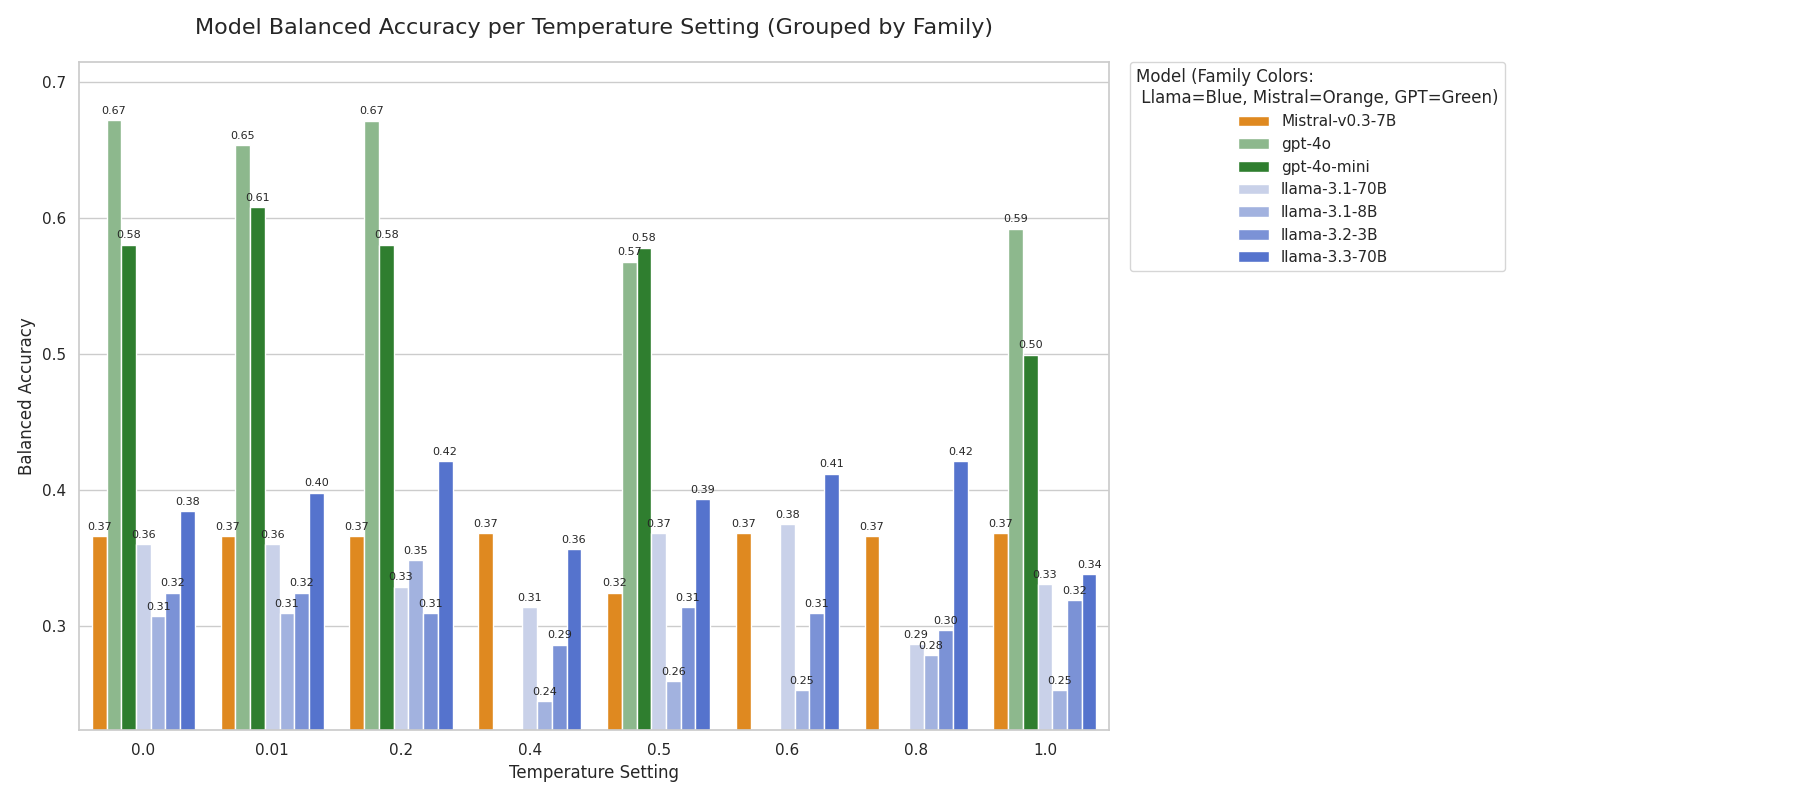
\includegraphics[width=10cm]{Graphs/Balanced Accuracy.png}
\end{figure}
\begin{figure}[H]
    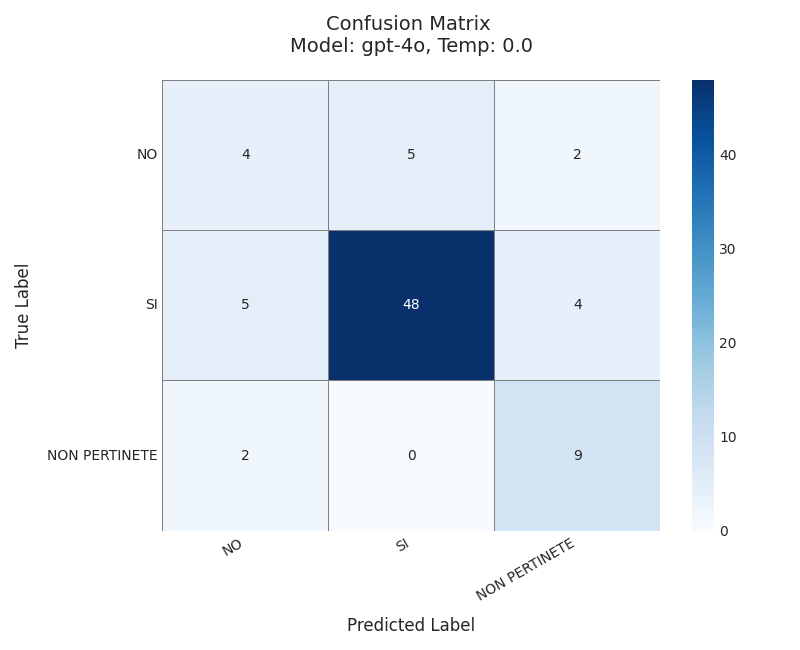
\includegraphics[width=10cm]{Graphs/Confusion Matrix GPT 4o.png}
\end{figure}
\begin{figure}[H]
    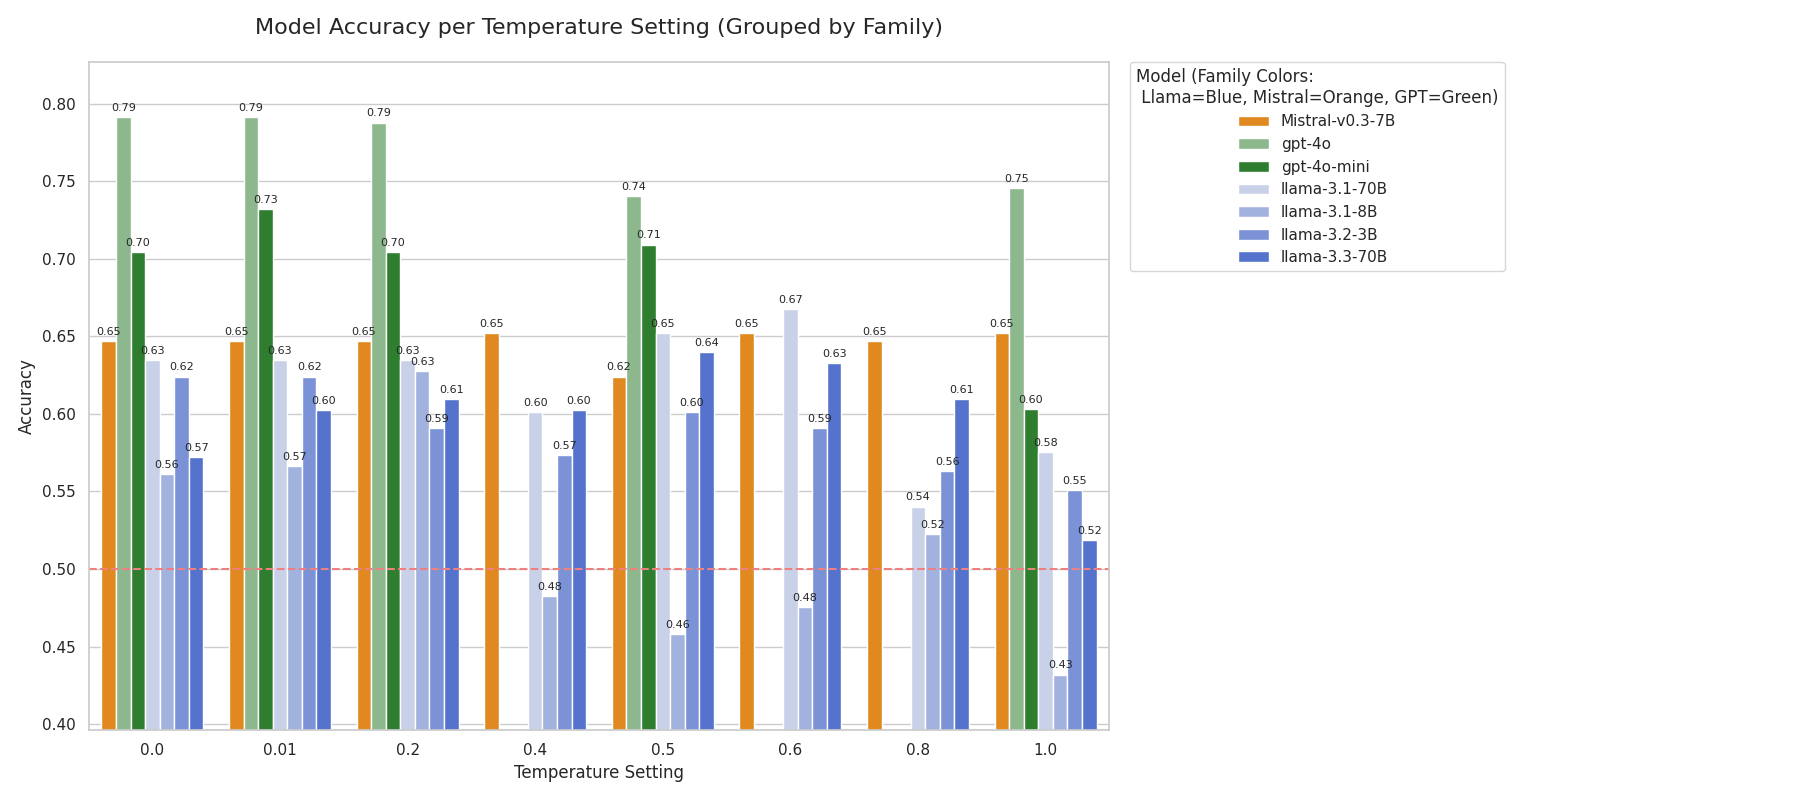
\includegraphics[width=10cm]{Graphs/Model Accuracy final.png}
\end{figure}

% Include bibliography only when compiling this subfile independently
\ifSubfilesClassLoaded{
    \bibliographystyle{sapthesis}
    \bibliography{Tesi}
}{}

\end{document}